\section{Experiments}\label{s:experiments}

We assess our methods against the relevant state of the art on standard benchmarks.

\paragraph{Data.}\label{s:expsetup}

For our experiments, we use the KITTI Object Detection dataset~\cite{geiger12are-we-ready} which has 7481 frames with labels in 3D\footnote{KITTI is provided with a Attribution-NonCommercial-ShareAlike 3.0 Unported License.
While KITTI contains images of pedestrians collected presumably without consent, they are often not large enough to be easily identifiable and no offensive content is included.}.
%{\color{red}Our method is used for auto-annotation, so in principle there is no need to split the data in a training and test/validation set.
However, we do so for compatibility with prior work.
% I've never been overly confident in making such claims wrt unsupervised methods, inter-frame similarity surely is very influential, as evidenced by our sequence-wise adaption
Specifically, we use the split found in~\cite{chen2017multiview}, the standard across all prior works which  first splits the videos into training and validation sets focusing on two different parts of the world (no visual overlap).
The network is learned on the training videos using multiple frames and then applied and evaluated on the validation videos on a single-frame basis.

% which separates examples based on the video sequences such that no areas seen in the training set are present in the validation set.
KITTI evaluates vehicle detectors using Birds Eye View (BEV) IOU and 3D box IOU (3D) with a strict cutoff of $0.7$ for a positive detection.
To be compatible with other relevant works in automated labelling~\cite{sdflabel, qin20weakly}, we evaluate instead at a threshold of $0.5$, also used for other KITTI categories, which reduces the influence of object size on IoU performance.
In part, this is motivated by~\cite{feng2020labels} which notes that the size of the `ground-truth' KITTI annotations are often imprecise due to the fact that many object instances have few LiDAR points and thus it is difficult for human annotators to accurately estimate metric size.
%  have  aa which points out the inherent ambiguity of LiDAR point clouds as an annotation reference as many objects in the KITTI dataset have a very sparse set of points available to annotate which may not lead to good size ground truth data owing to the partial nature of scans in the wild.
% }

% {\color{red}
% \begin{itemize}
%     \item Toyota takes 6 seconds to label a single instance on Titan V, 2 hours for whole dataset labelling on 2 gpus, I can benchmark Titan V on Aims server but titan rtx in desktop is faster anyways
%     \item we should also try online adapting
% \end{itemize}
% }

\paragraph{Data preprocessing.}

To construct our training set we first run Mask-RCNN~\cite{he17mask,wu2019detectron2} with the ResNet 101 backend to locate cars in the images.
We then extract the LiDAR points contained within the masks detected and use these for 3D labelling.
% For tracking between frames we take the median of the produced point clouds for robustness to outliers and compare this to detections in subsequent frames taking ego motion into account and retain only those which are sufficiently close to be the same car.
When tracking for 5 frames this gives us 9.6k cars in the training.
% We also require that the number of lidar points in subsequent frames not be significantly different than the previous as some Mask-RCNN detections are {\color{red} bad (not false positives but only include small parts of an object or a mask in the first frame contained multiple objects and another prediction was a single object then we want to match to the single object)} 
For evaluation we only use a single frame of Mask R-CNN detection and use the mask score as the confidence for our predictions.

\paragraph{Implementation.}

We implement our method in Pytorch\cite{NEURIPS2019_9015} and use components from Frustum PointNets\cite{qi2017frustum} to construct our network.
All variants are trained with Adam optimizer with a learning rate of $3\times 10^{-3}$ decreasing every 30 steps with multiplier $0.3$ for a total of 150 epochs with a batch size of 64 .
Training was performed on a single Titan RTX with a Ryzen 3900X processor and the most complex models had a training time of 7 hours.

% {\color{red}The use of negative log-likelihood of a factorised Laplacian distribution already improves the performance of our model significantly compared to the baseline using the loss derived from $\hat{d}$.When capturing LiDAR points withing a 2d detection frustum high occlusion can result in a very sparse low number of points which are hard to fit using our existing method.However when multiple frames are used the number of LiDAR points on the object of interest can change greatly allowing our model to make a more confident prediction.To utilise a variety of viewpoints across time we penalise our model for predictions where the estimated centre and yaw are inconsistent across time.

\begin{table}
\setlength{\tabcolsep}{1.5mm}
\centering
\begin{tabular}{c c c c c c c c c c}
\toprule
    & \multicolumn{3}{c}{Components} & \multicolumn{3}{c}{AP\textsubscript{BEV}(IoU = 0.5)} & \multicolumn{3}{c}{AP\textsubscript{3D}(IoU = 0.5)} \\
    & Filtering                      & Outlier-aware                                        & Multi-view                                            & Easy           & Moderate       & Hard           & Easy           & Moderate       & Hard \\
 \cmidrule(r){2-4}
 \cmidrule(lr){5-7}
 \cmidrule(l){8-10}
(a) & 2D Box                         &                                                      &                                                       & 35.53          & 41.54          & 33.96          & 23.79          & 28.32          & 23.12 \\
(b) & \cellcolor{green}2D Mask       &                                                      &                                                       & 58.61          & 62.56          & 54.20          & 53.40          & 57.02          & 48.04 \\
(c) & \cellcolor{green}2D Mask       &                                                      & \cellcolor{green}\checkmark                           & 58.63          & 61.70          & 54.11          & 51.22          & 52.91          & 47.19 \\
(d) & \cellcolor{green}2D Mask       & \cellcolor{green}\checkmark                          &                                                       & 75.46          & 76.60          & 68.59          & 69.59          & 70.35          & 62.81 \\
(e) & \cellcolor{green}2D Mask       & \cellcolor{green}\checkmark                          & \cellcolor{green}\checkmark                           & \textbf{81.34} & \textbf{81.82} & \textbf{73.77} & \textbf{74.96} & \textbf{75.53} & \textbf{68.11} \\
\bottomrule
\end{tabular}
\caption{Ablation of different components of the model and data processing steps. Our full model with automatic outlier removal and multi-view consistency achieves the highest accuracy.}\label{t:ablation}
\end{table}

\begin{table}
\centering
\begin{tabular}{c l c c c  c c c  }
\toprule
   &\multirow{2}{*}{Paradigm}                                 & \multicolumn{3}{c}{AP\textsubscript{BEV}(IoU = 0.5)} & \multicolumn{3}{c}{AP\textsubscript{3D}(IoU = 0.5)} \\
   &                                                          & Easy                                                 & Moderate                                              & Hard           & Easy           & Moderate       & Hard \\
\cmidrule(lr){2-2}
\cmidrule(lr){3-5}
\cmidrule(lr){6-8}
(a)& arctan                                             & 76.65                                                & 79.05                                                 & 69.33          & 74.85          & 75.36          & 65.81 \\
(b)&Insafutdinov \& Dosovitskiy~\cite{insafutdinov18pointclouds} & 77.28                                                & 76.92                                                 & 69.12          & 70.18          & 70.22          & 61.54 \\
(c)&Goel et al.~\cite{goel20shape}                            & 76.49                                                & 77.35                                                 & 69.69          & 68.43          & 69.62          & 62.83\\
\midrule
(d)&Ours, 16 bins       & 77.04                & 77.30              & 69.49          & 65.42          & 66.78          & 59.72 \\
(e)&Ours, 32 bins       & 79.93                & 81.14              & 73.15          & 74.96          & 75.53          & 68.11 \\
(f)&Ours, 64 bins       & \textbf{80.07}       & \textbf{82.23}     & \textbf{74.1} & \textbf{78.48} & \textbf{77.63} & \textbf{69.90} \\
(g)&Ours, 128 bins      & 81.79                & 82.23              & 74.11          & \textbf{78.49} & \textbf{77.68} & \textbf{69.86} \\
\bottomrule
\end{tabular}
\caption{Comparison of yaw prediction techniques.}\label{t:yaw}
\end{table}

\subsection{Ablations of model components}

We first start by analysing the individual components of our model (\cref{t:ablation}).
First, we do not use the 2D mask to filter LiDAR points, significantly increasing the number of outliers, arising in particular from cars proximal to the target one (row (a)).
% Our first experiment provides a baseline where all points inside a 2D bounding box (not using instance segmentation mask) are compared to %our subsampling of 
% the template mesh.
% In this case many cars can be occluded by other cars which results in inputs to the network with multiple cars that could be the correct answer.
Masking LiDAR points (row (b)) results in a substantial improvement, removing most of these outliers (see also \cref{fig:dataset_example}).
Introducing the temporal consistency/equivariance loss~\eqref{e:keypointloss} (row (c)) does not give by itself a noticeable benefit because outlier points are still heavily influential to the prediction.
Discounting outliers using the probabilistic formulation of \cref{e:distance} increases accuracy substantially (row (d)).
Furthermore, bringing back the consistency loss, which amounts to our full model, does now show a significant benefit (row (e)).
Our interpretation is that considering multiple frames can significantly aid discovering and learning outlier patterns:
this is because outliers tend to be \emph{inconsistent} across frames, so reasoning over multiple frames helps discovering them (see \cref{fig:multiframe_example}).
% Notably, multi-view training does help significantly when trained with outlier exclusion, as in the single frame case this network can minimize to the largest cluster of points whereas in cases as seen in \cref{fig:multiframe_example} the network is influenced by the consistency between frames where other frames may have a better set of points to be fit.

\paragraph{Yaw estimation.}

In \cref{t:yaw} we evaluate our approach for estimating camera viewpoint proposed in \cref{s:direct-yaw}.
% The comparison is shown  where we vary the number of bins into which we discretise the yaw angle while the rest of the settings correspond to our full model (Outlier-aware + multi-view).
First we experiment with a network $\Phi$ tasked to output a vector $\mathbf{x} \in \mathbb{R}^2$ with the yaw angle computed as $\theta = \arctan(x_1/x_2)$ (row (a)).
Our direct prediction approach (rows (d-g)) outperforms this na{\:\i}ve baseline by a significant margin.
Our method is influenced by the number of discrete rotations, 64 being optimal (row (f)).
% For our metwith the gap growing as the number of bins increases.
% Using 64 bins achieves the best results while the further refinement provides only diminishing returns.
In order to provide stronger baselines, we additionally implement to alternative techniques~\cite{insafutdinov18pointclouds,goel20shape} to handle ambiguous predictions in 3D pose estimation, but did not observe a benefit (rows (b) and (c)) compared to simple direct arctan regression.
This is perhaps due to the different setting (\cite{insafutdinov18pointclouds,goel20shape} were proposed to handle ambiguous fitting of 3D shapes to 2D silhouettes).

% These baselines perform comparably with our approach under coarse discretisation, however the difference in accuracy becomes significant when the number of bins is $32$ or greater.
% The prior methods were developed for the downstream task of fitting 3D shapes to 2D silhouettes and we hypothesise that they are not as effective when applied in our setting as our target vehicles are much smaller in the image.
% Predicting yaw for unconstrained 3d objects results in a discontinuity at the angle where the prediction range starts/ends.

% Supervised methods typically rely on classification or prediction of a vector or quaternion, both of which can be adapted to our.

\subsection{SoTA comparison}

In \cref{t:averageprecision} we compare our method to the relevant state of the art.
% Comparing to other methods on the same task and dataset we see that our method easily bests the existing weakly supervised methods (\cref{t:averageprecision}).
VS3D~\cite{qin20weakly} uses a viewpoint estimation network pretrained on Pascal 3D and NYC 3D cars~\cite{xiang_wacv14, MatzenICCV13} with ground truth yaw annotations.
In Zakharov~\cite{zakharov20autolabeling} a synthetic dataset is used to initialise a coordinate shape space NOCS~\cite{Wang_2019_CVPR} providing a strong prior on 3D shape and yaw estimation.
During fitting stage they only utilise Mask R-CNN predictions which have a large overlap with ground truth 2D boxes and also takes 6 seconds to infer a single car on a modern GPU making it infeasible for real time prediction unlike VS3D~\cite{qin20weakly} (22Hz) and our method which runs at 200Hz after the 2D object detection method (about 25Hz).
Frustum PointNet~\cite{qi2017frustum} is a fully supervised method trained on KITTI that serves as a reference with similar architecture to our own method.
It should be noted that the 2D predictions generated by Frustum PointNets are significantly higher (10\%+) than our own as a result of its training specifically on cars in the KITTI dataset.
However, this is not so much due to imperfections in our weakly-supervised prediction, but more to the fact that our 2D detector is trained on COCO~\cite{lin2014microsoft} and picks up more vehicle classes than just cars, with this detections being accounted as false positives in this evaluation.
%  objects and False Positives which negatively impacts performance both directly in the AP metric and indirectly in that it provides bad training examples.


% Comparing to other methods on the same task and dataset we see that our method easily bests the existing weakly supervised methods (\cref{t:averageprecision}).

% timing by preloading the Mask-rcnn into ram and running detectron2 only in a separate loop

% \begin{table*}[t]
\newcommand{\zero}{ZERO}
\centering

\resizebox{\textwidth}{!}{
\setlength{\tabcolsep}{1.8mm}{
\begin{tabular}{c | c | c c | c | c c c }
 \toprule
 \multirow{2}{*}{Paradigm} & \multirow{2}{*}{Method} & \multicolumn{2}{c}{External Data Supervision} & & \multicolumn{3}{c}{AP\textsubscript{BEV}~/~AP\textsubscript{3D} (IoU = 0.5)} \\
 & & COCO 2D Detection & Pascal3d & Kitti GT 2D Boxes & Easy & Moderate & Hard \\\hline


% \multirow{3}{*}{\textit{\makecell{ Weakly \\ supervised}}}
%   &PCL~\cite{tang2018pcl}      &  & & & 1.878 /- &1.058 /- &0.935 /- \\
%   &OICR~\cite{tang2017oicr}    &  & & & 6.481 /- &2.933 /- &3.270 /- \\
%   &MELM~\cite{wan2018min}      &  & & & 2.796 /- &1.486 /- &1.476 /- \\
%     \hline

\multirow{1}{*}{\textit{\makecell{Supervised}}}
  &Frustum PointNet~\cite{qi2017frustum}      & & & & 98.25/98.10 & 94.92/94.31 & 87.14/86.48 \\
    \hline

%   &VS3D\cite{meng2020ws3d} & Mono   & 2d box,Yaw & 76.93 / 31.35 & 71.84 / 23.92 & 59.39 / 19.34 \\
%   &VS3D\cite{meng2020ws3d} & Stereo & 2d box,Yaw & 79.03 / 40.98 & 72.71 / 34.09 & 59.77 / 27.65 \\

  
   
   
%   &VS3D\cite{meng2020ws3d} & Mono + LiDAR    & Yaw from Image & 81.60 / 41.83 & 72.43 / 39.22 & 64.31 / 32.73 \\
%   &VS3D\cite{meng\2020ws3d} & Stereo + LiDAR  & Yaw from Image & 81.95 / 42.43 & 73.21 / 41.58 & 64.34 / 32.74 \\
%   \hline
  &VS3D\cite{meng2020ws3d} &  & \cellcolor{green} 2D Detection, Yaw & & 74.54 / 40.32 & 66.71 / 37.36 & 57.55 / 31.09 \\ 
  
  
\multirow{3}{*}{\textit{\makecell{Unsupervised}}}
   &Zakharov et al. \cite{sdflabel} & \cellcolor{green}\checkmark & & \cellcolor{green}\checkmark & 77.84/62.25 & 59.75/42.23 & -/- \\
   % Cremers paper here?
   
   &Ours &\cellcolor{green}\checkmark & &  & \textbf{82.37}/\textbf{78.48} & \textbf{82.57}/\textbf{77.63} & \textbf{74.40}/\textbf{69.90} \\
   
\end{tabular}}} 
\label{t:averageprecision}

\caption{Object Detection Average-Precision on the Kitti validation set. Compared to our Method VS3D\cite{meng2020ws3d} uses a network trained on Pascal 3D and NYC 3D Cars\cite{xiang_wacv14, MatzenICCV13} to determine the object Yaw and 2D box, while while Zakharov\cite{sdflabel} only considers MASK R-CNN detections with an IOU > $50\%$ compared to a ground truth box and uses a synthetic dataset to train a network which gives yaw.}

\end{table*}
\begin{table*}[t]
\newcommand{\zero}{ZERO}
\centering
\setlength{\tabcolsep}{1mm}
\begin{tabular}{cc c c c  c c c}
\toprule
&\multirow{3}{*}{Method} & \multicolumn{3}{c}{Annotations Source} & \multicolumn{3}{c}{AP\textsubscript{BEV}~/~AP\textsubscript{3D} (IoU = 0.5)} \\
&& \textbf{2D} & \multicolumn{2}{c}{\textbf{3D}}  \\
&& Boxes & Yaw & Boxes & Easy & Moderate & Hard \\
\cmidrule(r){1-2}
\cmidrule(lr){3-3}
\cmidrule(lr){4-5}
\cmidrule(l){6-8}
% \multirow{3}{*}{\textit{\makecell{ Weakly \\ supervised}}}
%   &PCL~\cite{tang2018pcl}      &  & & & 1.878 /- &1.058 /- &0.935 /- \\
%   &OICR~\cite{tang2017oicr}    &  & & & 6.481 /- &2.933 /- &3.270 /- \\
%   &MELM~\cite{wan2018min}      &  & & & 2.796 /- &1.486 /- &1.476 /- \\
%     \hline
%   &VS3D\cite{meng2020ws3d} & Mono   & 2d box,Yaw & 76.93 / 31.35 & 71.84 / 23.92 & 59.39 / 19.34 \\
%   &VS3D\cite{meng2020ws3d} & Stereo & 2d box,Yaw & 79.03 / 40.98 & 72.71 / 34.09 & 59.77 / 27.65 \\
%   &VS3D\cite{meng2020ws3d} & Mono + LiDAR    & Yaw from Image & 81.60 / 41.83 & 72.43 / 39.22 & 64.31 / 32.73 \\
%   &VS3D\cite{meng\2020ws3d} & Stereo + LiDAR  & Yaw from Image & 81.95 / 42.43 & 73.21 / 41.58 & 64.34 / 32.74 \\
%   \hline
(a) &VS3D~\cite{meng2020ws3d} & Pascal 3D & NYC Cars & & 74.5/40.32 & 66.71/37.36 & 57.55/31.09 \\
\hline
(b) &Zakharov et al. \cite{sdflabel} & KITTI & KITTI &  & 77.84/62.25 & 59.75/42.23 & -/- \\
% Cremers paper here?
% (c) &\textbf{ours} &MS-COCO & &  & \textbf{80.73±2.64}/\textbf{76.73±2.4} & \textbf{81.70±1.29}/\textbf{76.66±1.23} & \textbf{73.61±1.11}/\textbf{69.01±1.03} \\
\hline
(c) &\textbf{ours} &MS-COCO & &  & \multirowcell{2}{\textbf{80.73}±2.64/\\ \textbf{76.73}±2.4} & \multirowcell{2}{\textbf{81.70}±1.29/\\ \textbf{76.66}±1.23} & \multirowcell{2}{\textbf{73.61}±1.11/\\ \textbf{69.01}±1.03} \\
\\
\hline
(d) &\textit{Frus.PointNet~\cite{qi2017frustum} }     & \textit{KITTI} & \textit{KITTI} & \textit{KITTI} & \textit{98.25/98.10} & \textit{94.92/94.31} & \textit{87.14/86.48} \\
\bottomrule
\end{tabular}
\caption{Object Detection Average-Precision on the Kitti validation set. Compared to our Method VS3D\cite{meng2020ws3d} uses a network trained on Pascal 3D and NYC 3D Cars\cite{xiang_wacv14, MatzenICCV13} to determine the object Yaw and 2D box, while while Zakharov\cite{sdflabel} only considers MASK R-CNN detections with an IOU > $50\%$ compared to a ground truth box and uses a synthetic dataset to train a network which gives yaw. We provide a 95\% confidence interval for our results using a variety of seeds. }\label{t:averageprecision}
\end{table*}
\begin{figure}
    \centering
    \begin{tabular}{c c}
        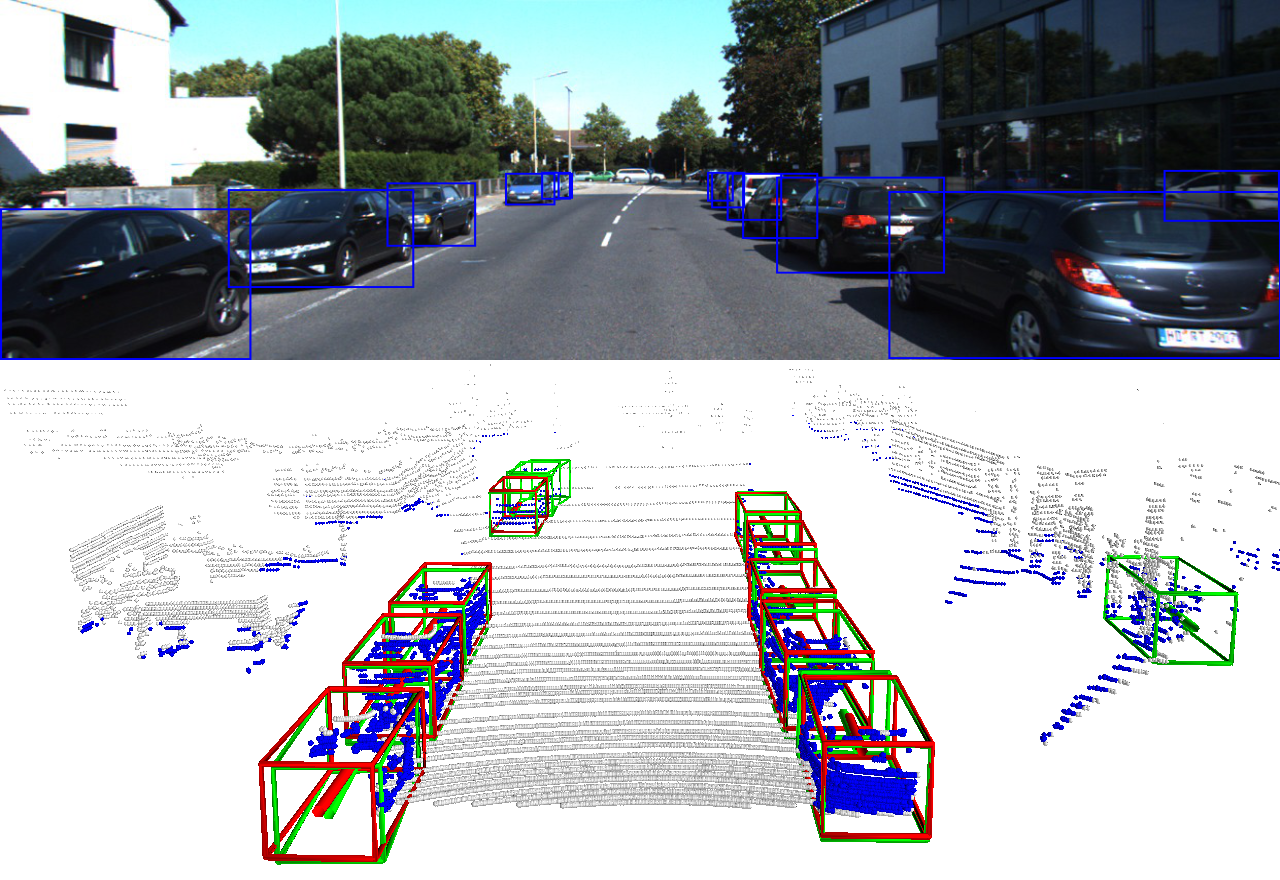
\includegraphics[width=0.5\textwidth]{figures/Qualitative_examples/314.png} & 
        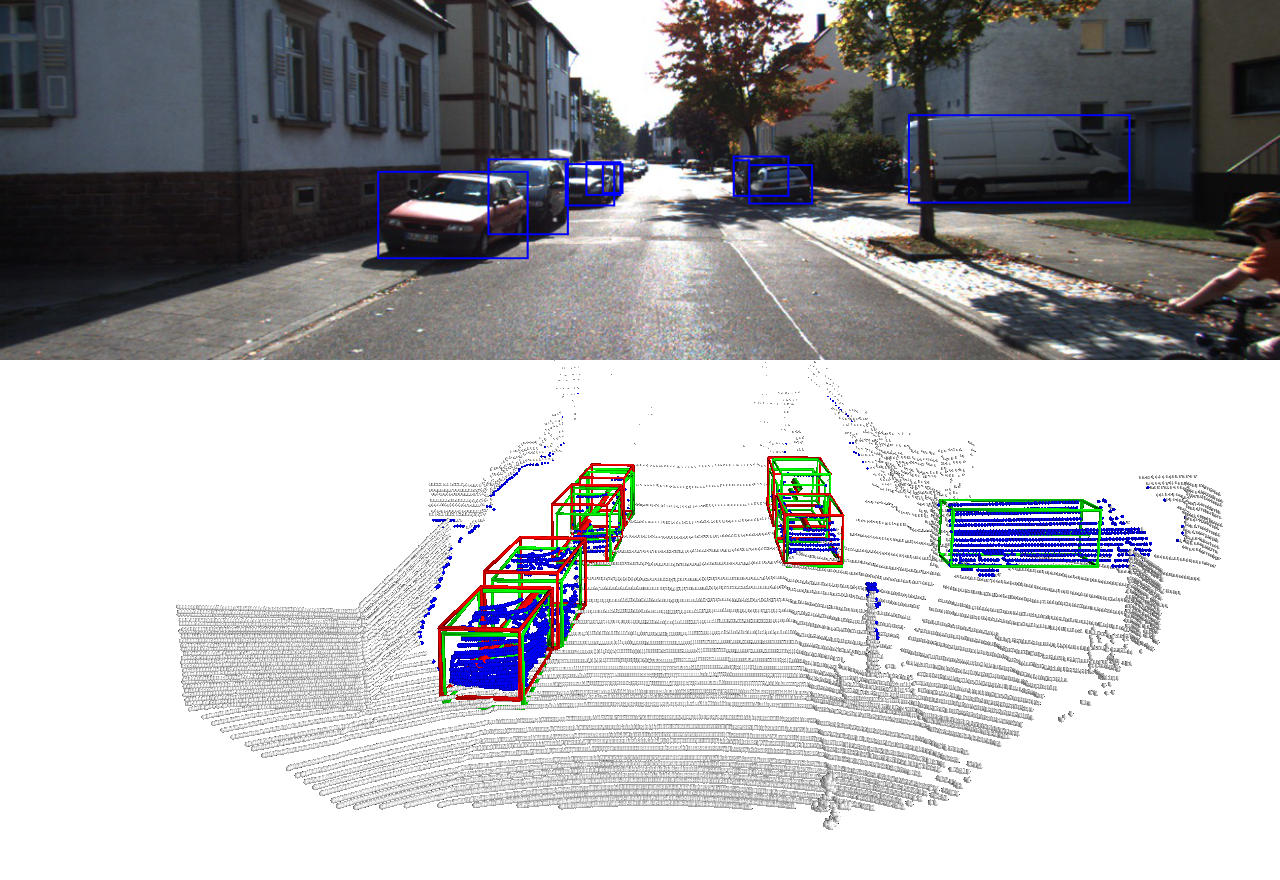
\includegraphics[width=0.5\textwidth]{figures/Qualitative_examples/245.png} \\
        % 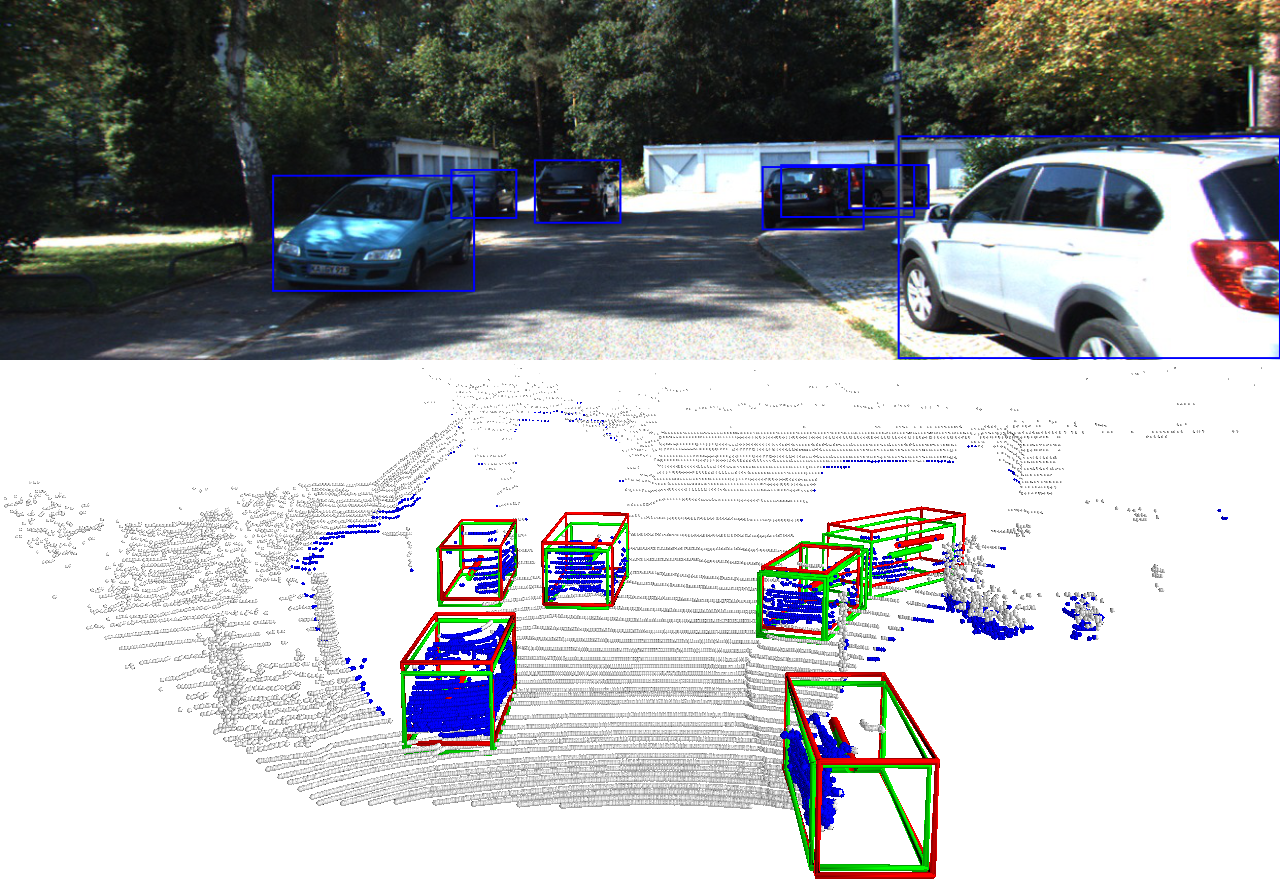
\includegraphics[width=0.5\textwidth]{figures/Qualitative_examples/217.png} 
        %  &  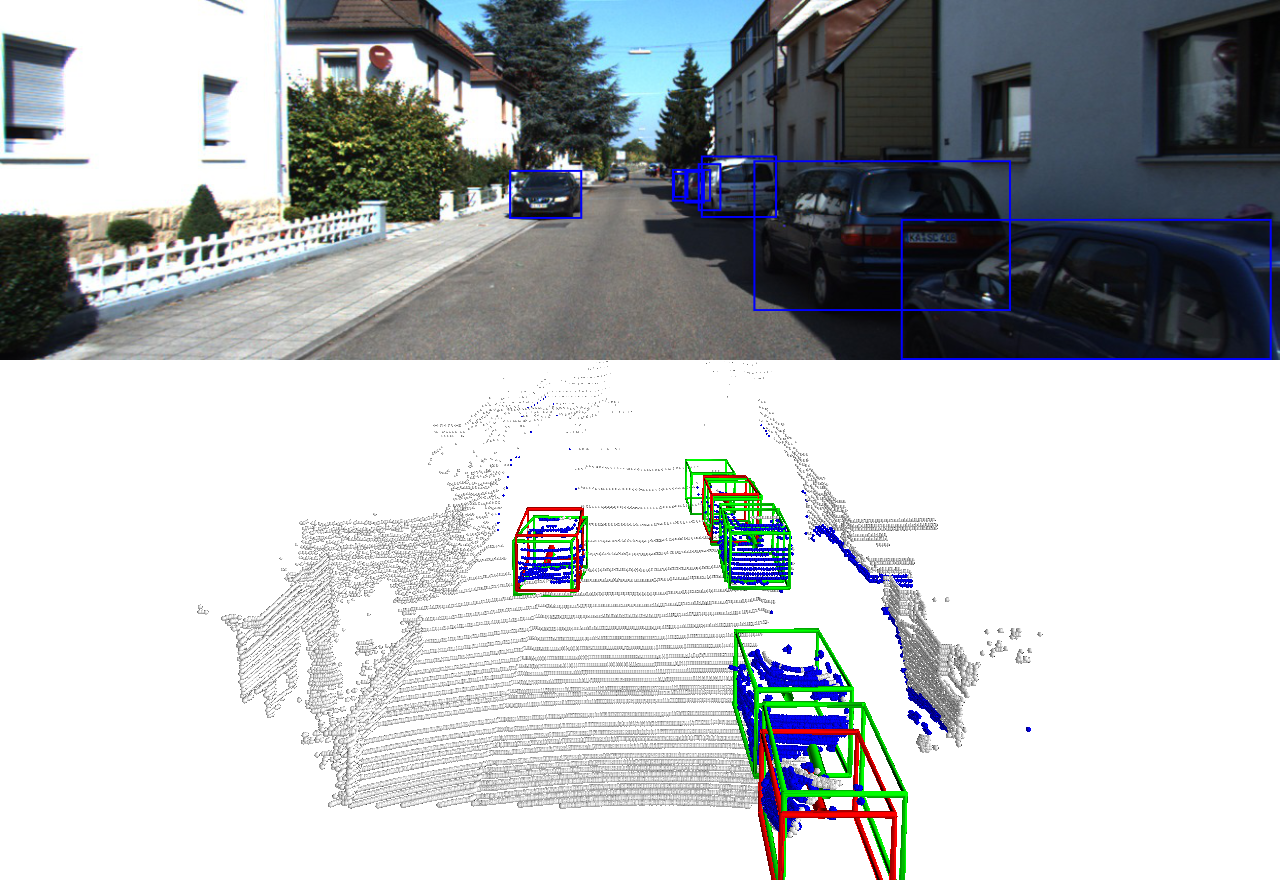
\includegraphics[width=0.5\textwidth]{figures/Qualitative_examples/178.png} \\
         
        % 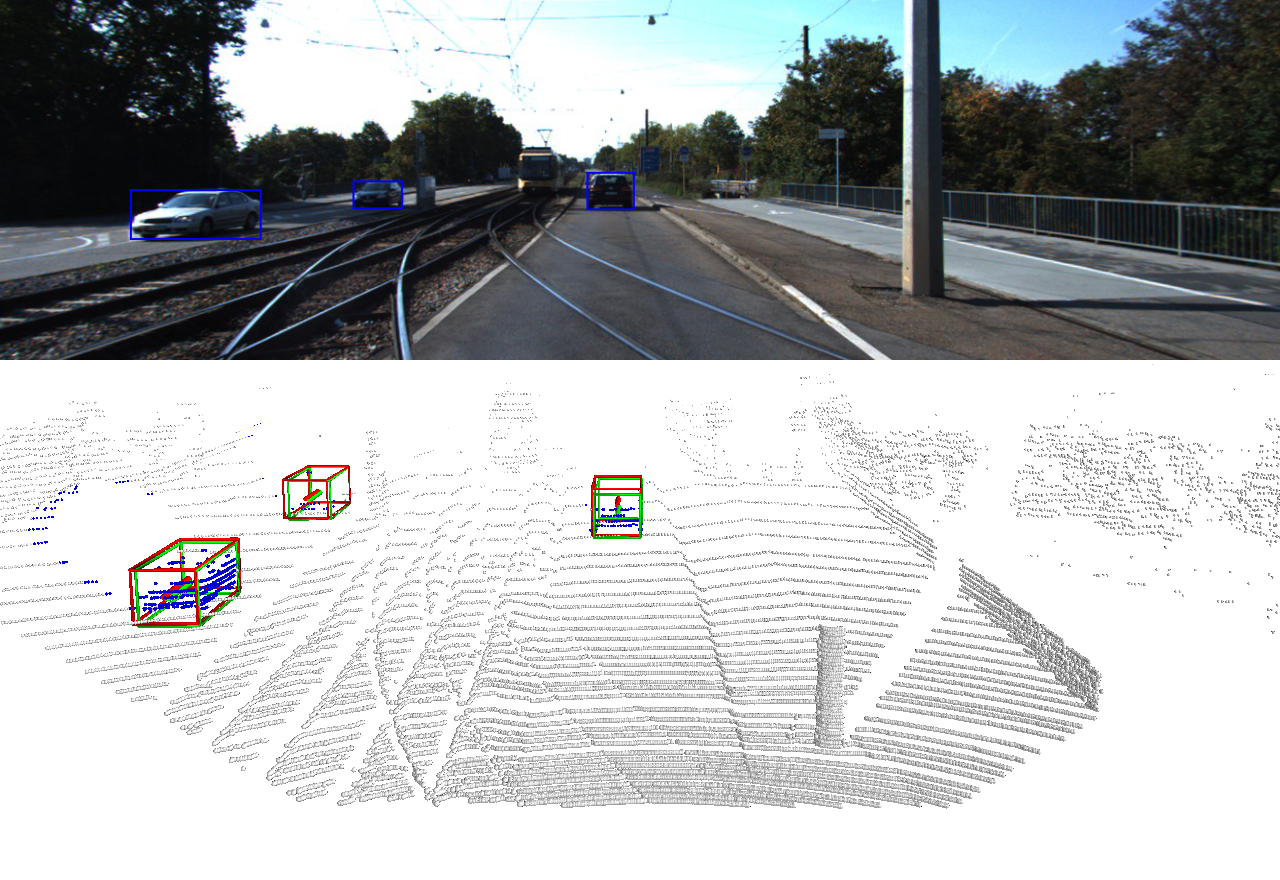
\includegraphics[width=0.5\textwidth]{figures/Qualitative_examples/172.png} & 
        % 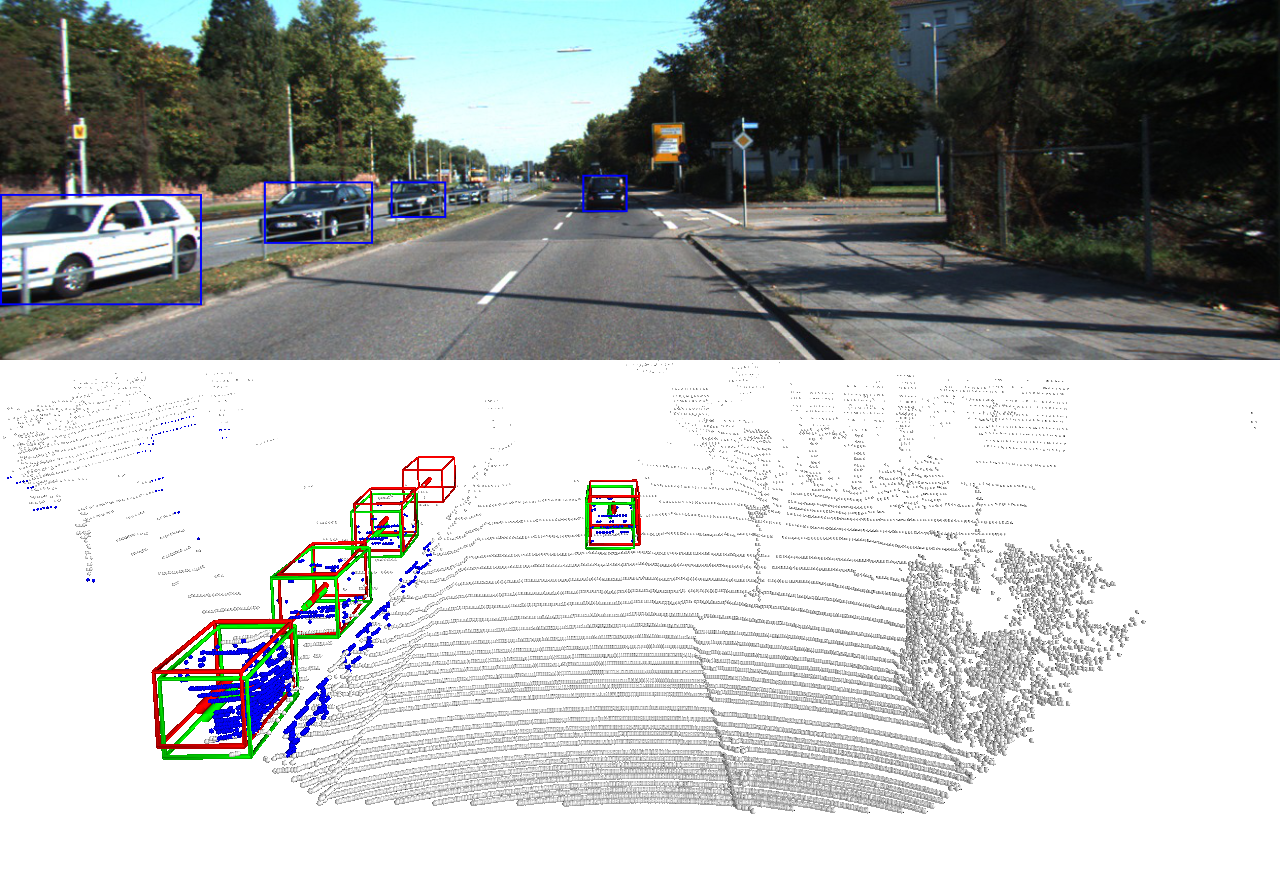
\includegraphics[width=0.5\textwidth]{figures/Qualitative_examples/52.png} \\
        
        % \includegraphics[width=0.5\textwidth]{figures/Qualitative_examples/171.png}
        %  &  \includegraphics[width=0.5\textwidth]{figures/Qualitative_examples/241.png} \\
 

        
    \end{tabular}
    \caption{Qualitative results of our method (green) on the Kitti Validation Set with ground truth car annotations in red and points inside each mask in blue.}
    \label{f:Qualitative}
\end{figure}
% \pgfplotstableread{
x       y      y-max  y-min
Easy  79.93 4.16 1.89
Medium 81.14 1.05  1.29
Hard 73.15 0.94 0.92    
}{\mytable}

\begin{figure}
    \centering
    \begin{tikzpicture}
        \begin{axis} [
                ymin=70,
                rotate=90,
                height=8cm,
                width=3cm,
                symbolic x coords={Easy, Medium, Hard},
                xtick=data,
                yticklabel pos=left,
                xticklabel pos=top,
                xticklabel style={left},
                yticklabel style={top},
                x dir=reverse,
                y dir=reverse
            ]
            \addplot [only marks] 
              plot [error bars/.cd, y dir=both, y explicit]
              table [y error plus=y-max, y error minus=y-min] {\mytable};
            \end{axis} 
    \end{tikzpicture}

    \caption{Error bars showing the variance of our method with 32 yaw bins with varying random seeds with the average, minimum and maximum shown for 14 runs.}
    \label{fig:error_bar}
\end{figure}
